\section{Laboratory work implementation}

\subsection{Tasks and Points}
Basic Level:

    - Create a Windows application what will display a dialog box on some event (ex. on clicking some button)
    
    - Add a system menu to your application with at least 3 items (add actions to that items)
   
    - Hook keyboard input. Add 2 custom events for 2 different keyboard combinations


Normal Level:

    - Realize the tasks from Basic Level.

    - Add 2 scroll bars that will manage main window size or position



\subsection{Laboratory work analysis}
Repository:

https://github.com/StasBizdiga/WP

\subsection{Proving my work}

Features:

- On clicking the MICRO button, the window shrinks to its minimal size. It then displays a dialog box as required by the first task.



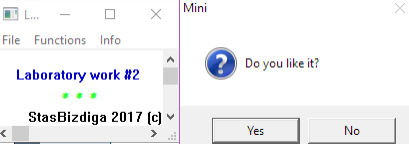
\includegraphics{pic_1}


- There are system menus with different actions to them:


Menu - Exit 	   : exits the window

Functions - Micro  : makes the window smallest possible

Functions - Center : moves the window to the middle of the screen

Info - About		: displays an "about" joke message box

Info - Help			: displays a help joke message box


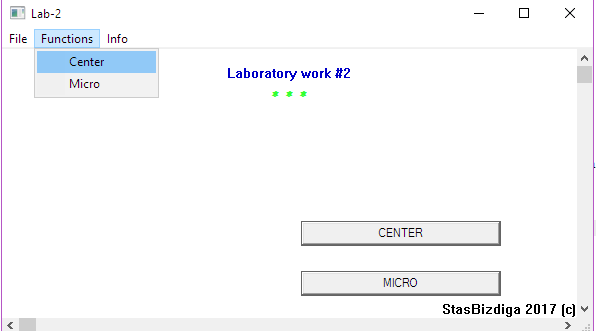
\includegraphics{pic_2}


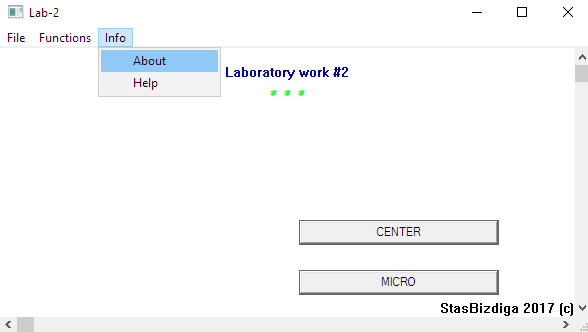
\includegraphics{pic_3}


- When pressing Shift and then any arrow key: UP,DOWN,LEFT,RIGHT you get a message depending on which key you pressed. Here I press SHIFT+RIGHT:


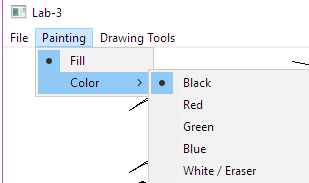
\includegraphics{pic_4}


- Scroll bars are used to move and resize the window:


Vertical scrolling: moves window to a constant position (top-left: x=0,y=0)

Horizontal scrolling: resizes the window to a constant of x=300 y=300




\clearpage